\subsubsection{Encapsulation and Atomicity}
Encapsulation means each actor has its own state, and thus all changes to the state of an actor has to come in a message sent from another actor. The notion of encapsulation is also one of the corner stones of object oriented programming where each object also has its own state. This can be very useful to enforce an object oriented decomposition in code, and may make actors look a lot like objects \cite{ActorModelPaper}.\\
Encapsulation has also lead to the notion of atomicity. In a sequential program one object may call a method in another object. This method will then run to the end before another object can call the method again. The called object may or may not have changed state during the method call, but we can only reason about this because the method call can not be interrupted by another method call. Because all method calls are run uninterrupted, we can reason about the object's behaviour given we know its state prior to the method call \cite{ActorModelPaper}.\\
In a concurrent setting an object may call a method in another object, but right after a third object does the same. If the first method call would be interrupted to accommodate the second, the object's state might already be altered, and we can no longer reason about the behaviour the object exhibits after a call to its method. This would lead to inconsistencies in the system as these concurrent calls can happen at any time. To guarantee we can reason about object behaviour in actors we therefore must guarantee that received messaged are handled atomically, meaning that the processing of a message happens in one step, and is not interrupted by new messages. This ensures that the encapsulated state is consistent throughout the execution of a program \cite{ActorModelPaper}.

\subsubsection{Fairness}
The notion of fairness states that all actors are scheduled time to run, and that they will make progress given they have computations to do. It also states that all messages are guaranteed to reach their destination unless that actor has been permanently disabled. The notion of fairness allows us to reason about the liveness properties of actor programs \cite{ActorModelPaper}. Here we note that an actor program is started by an external message sent to an actor, and that an actor program terminates when all actors are idle and no external message can be passed to any actors. An actor is considered idle if it has no pending messages in its mailbox.

\subsubsection{Location transparency}
Location transparency provides an abstraction for the programmers who need to make actors communicate. In the actor model the location of actors does not determine its name. Two actors might run on the same computer in the same core, or they might run on two different machines in two different countries. Location transparent naming enables the programmers no to worry about the actors physical location. \cite{ActorModelPaper}.\\
Mobility is defined as the ability for a computation to migrate to another node \cite{ActorModelPaper}. This is important for load-balancing, fault-tolerance, and reconfiguration, and is useful in achieving scalable performance \cite{ActorModelPaper} as an actor lifting a lot of heavy work along other actors doing the same on the same machine can seamlessly be moved to another machine in an attempt to alleviate the workload on that machine.

\subsubsection{Synchronization}
\begin{figure}[H]
	\centering
	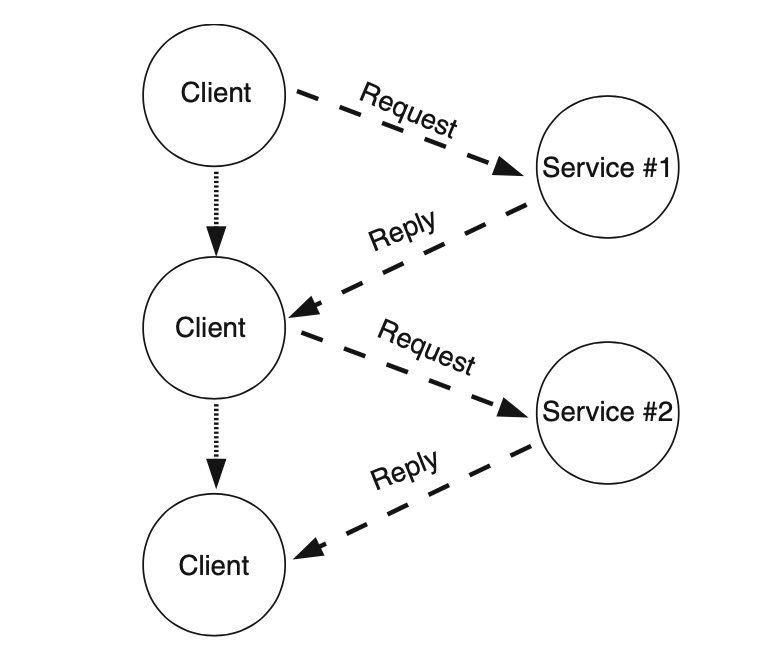
\includegraphics[width=0.6\linewidth]{Materials/ActorModel/AMCommunication}
	\caption{An illustration of how RPC like communication works. Figures is from \cite{ActorModelPaper}.}
	\label{AMCommunication}
\end{figure}
One way to achieve synchronization of actors is through Remote Procedure Call like message passing (RPC), which is a common communication pattern in actor systems \cite{ActorModelPaper}. In a situation where an actor wants to make sure another actor has received its message before it communicates it to others or where the order of messages matter RPC like messaging is a big help. In RPC like communication the sender of a message waits for a reply before it continues to process other messages. An actor might want to wait for a reply if it needs the information in the reply to continue its computation. This can be seen in \autoref{AMCommunication} where the client sends a message to a service and waits for the reply before sending another message to another service \cite{ActorModelPaper}.\\
